\subsubsection{Training-Accuracy Transformer Capacity}
\label{app:exp:additional:train99-capacity}

In~\Cref{fig:appendix:transformer-capacity-train99}, we rerun the main-text Transformer capacity experiment from Figure~\ref{fig:main-figure}c, but with a 99\% \emph{training accuracy} criterion instead of fact-adaptive accuracy (as defined in \Cref{appendix:lm-scaling}).
Unlike the evaluation accuracy plot, we fix the hidden dimension \(m\in\{44,88,176,352,704,1408\}\) and binary-search for the maximum number of facts \(F \in [1, 65536] \) that the Transformer is able to store.

\begin{figure}[t]
\centering
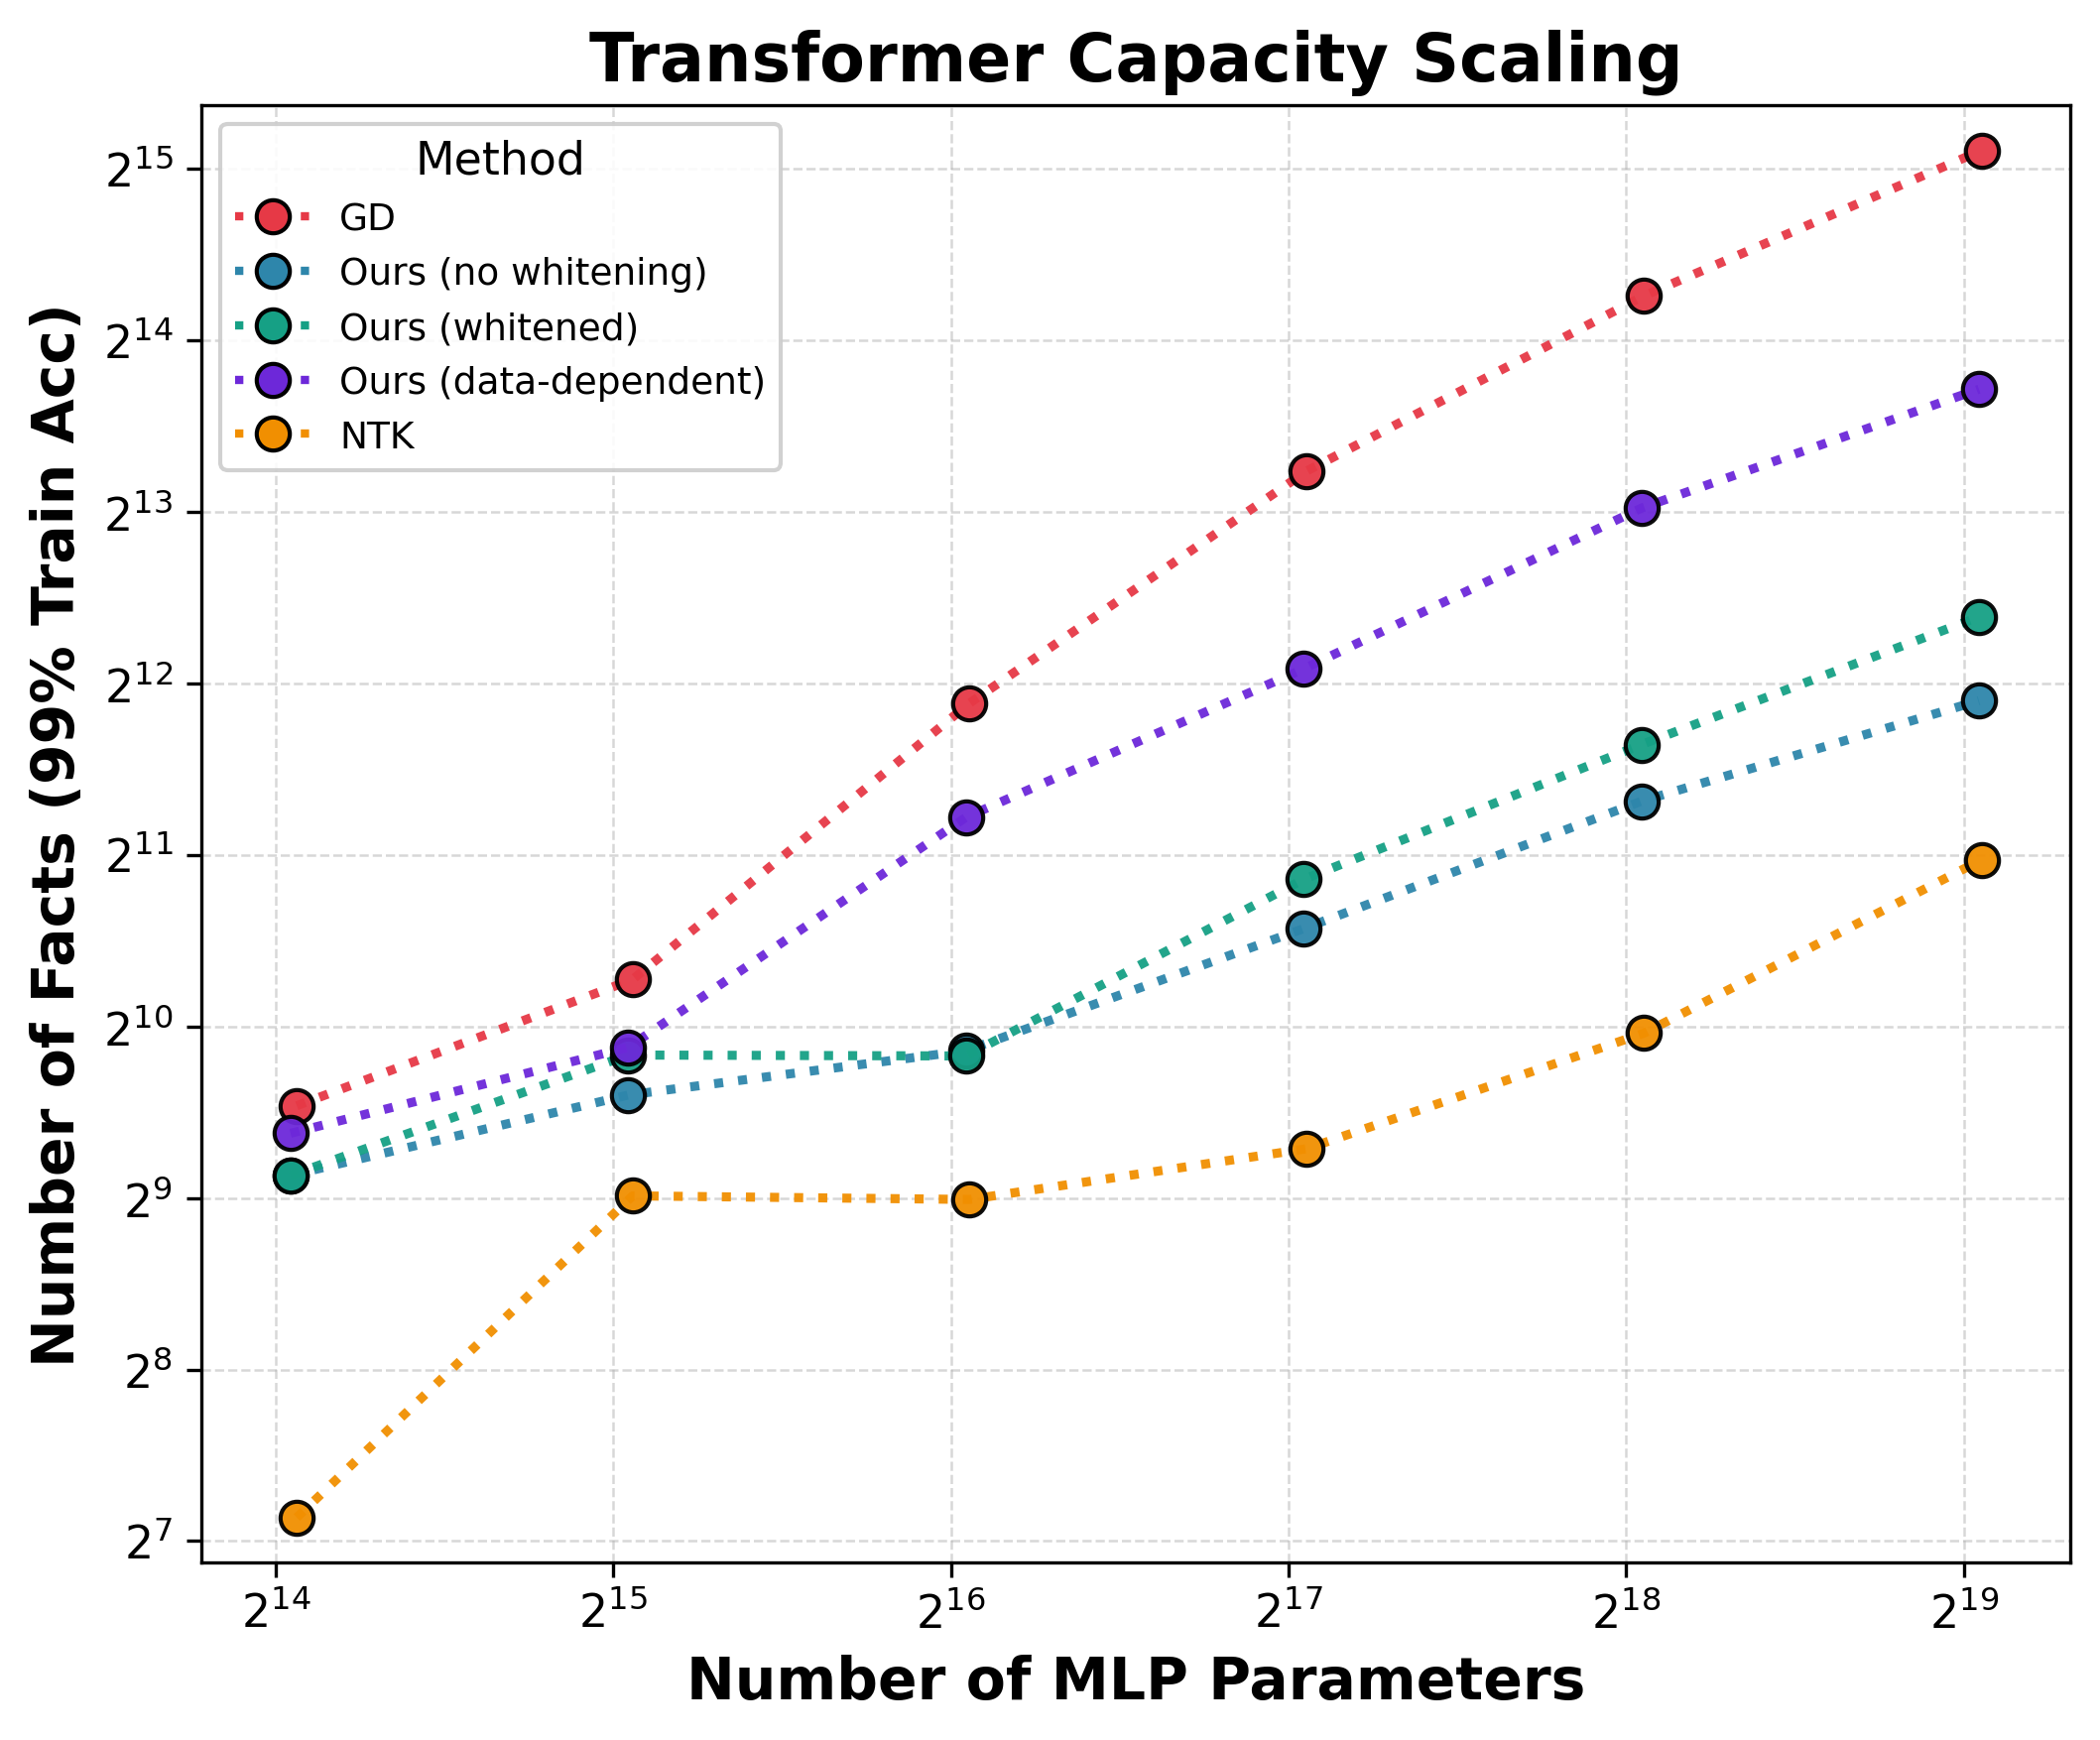
\includegraphics[width=0.78\linewidth]{sections/section_5_transformer_integration/figs/transformer_capacity_scaling_train99.png}
\caption{\textbf{Transformer fact-storage capacity under a 99\% training accuracy criterion.}
Transformer train-accuracy capacity is $2$-$8\times$ higher than fact-adaptive capacity for our constructions and fixes the asymptotics for NTK -- this suggests that attention parameters are learning to participate in storing the fact set.}
\label{fig:appendix:transformer-capacity-train99}
\end{figure}

Relative to the fact-adaptive frontier in Figure~\ref{fig:main-figure}c, the train-side plot stores roughly \(2\)–\(8\times\) more facts at a fixed parameter budget for GD MLPs and for all of our construction variants. The gaps close the most for the weakest constructions, especially NTK and our unwhitened method; in particular, the suboptimal fixed-\(d\) asymptotics of the NTK construction are avoided under the train-accuracy criterion.
This suggests that without the stricter fact-adaptive criterion, the surrounding attention layer uses its parameters to help store the fact set, rather than solely relying upon the inserted fact-storing MLP.

\subsubsection{Anisotropic MLP Capacity}
\label{app:exp:additional:anisotropic-mlp-capacity}

\Cref{fig:appendix:anisotropic-mlp-capacity} uses the same MLP capacity protocol as Appendix~\ref{app:exp:section4:capacity}, but evaluates the different MLP families on \emph{anisotropic} keys and values.
We apply the rank-1 spike model from Appendix~\ref{app:exp:section4:anisotropic-keys-values} with \(\beta=1.5\).
We then estimate the resulting fact-storage frontier for \(d\in\{64,90,128\}\).

\begin{figure}[t]
\centering
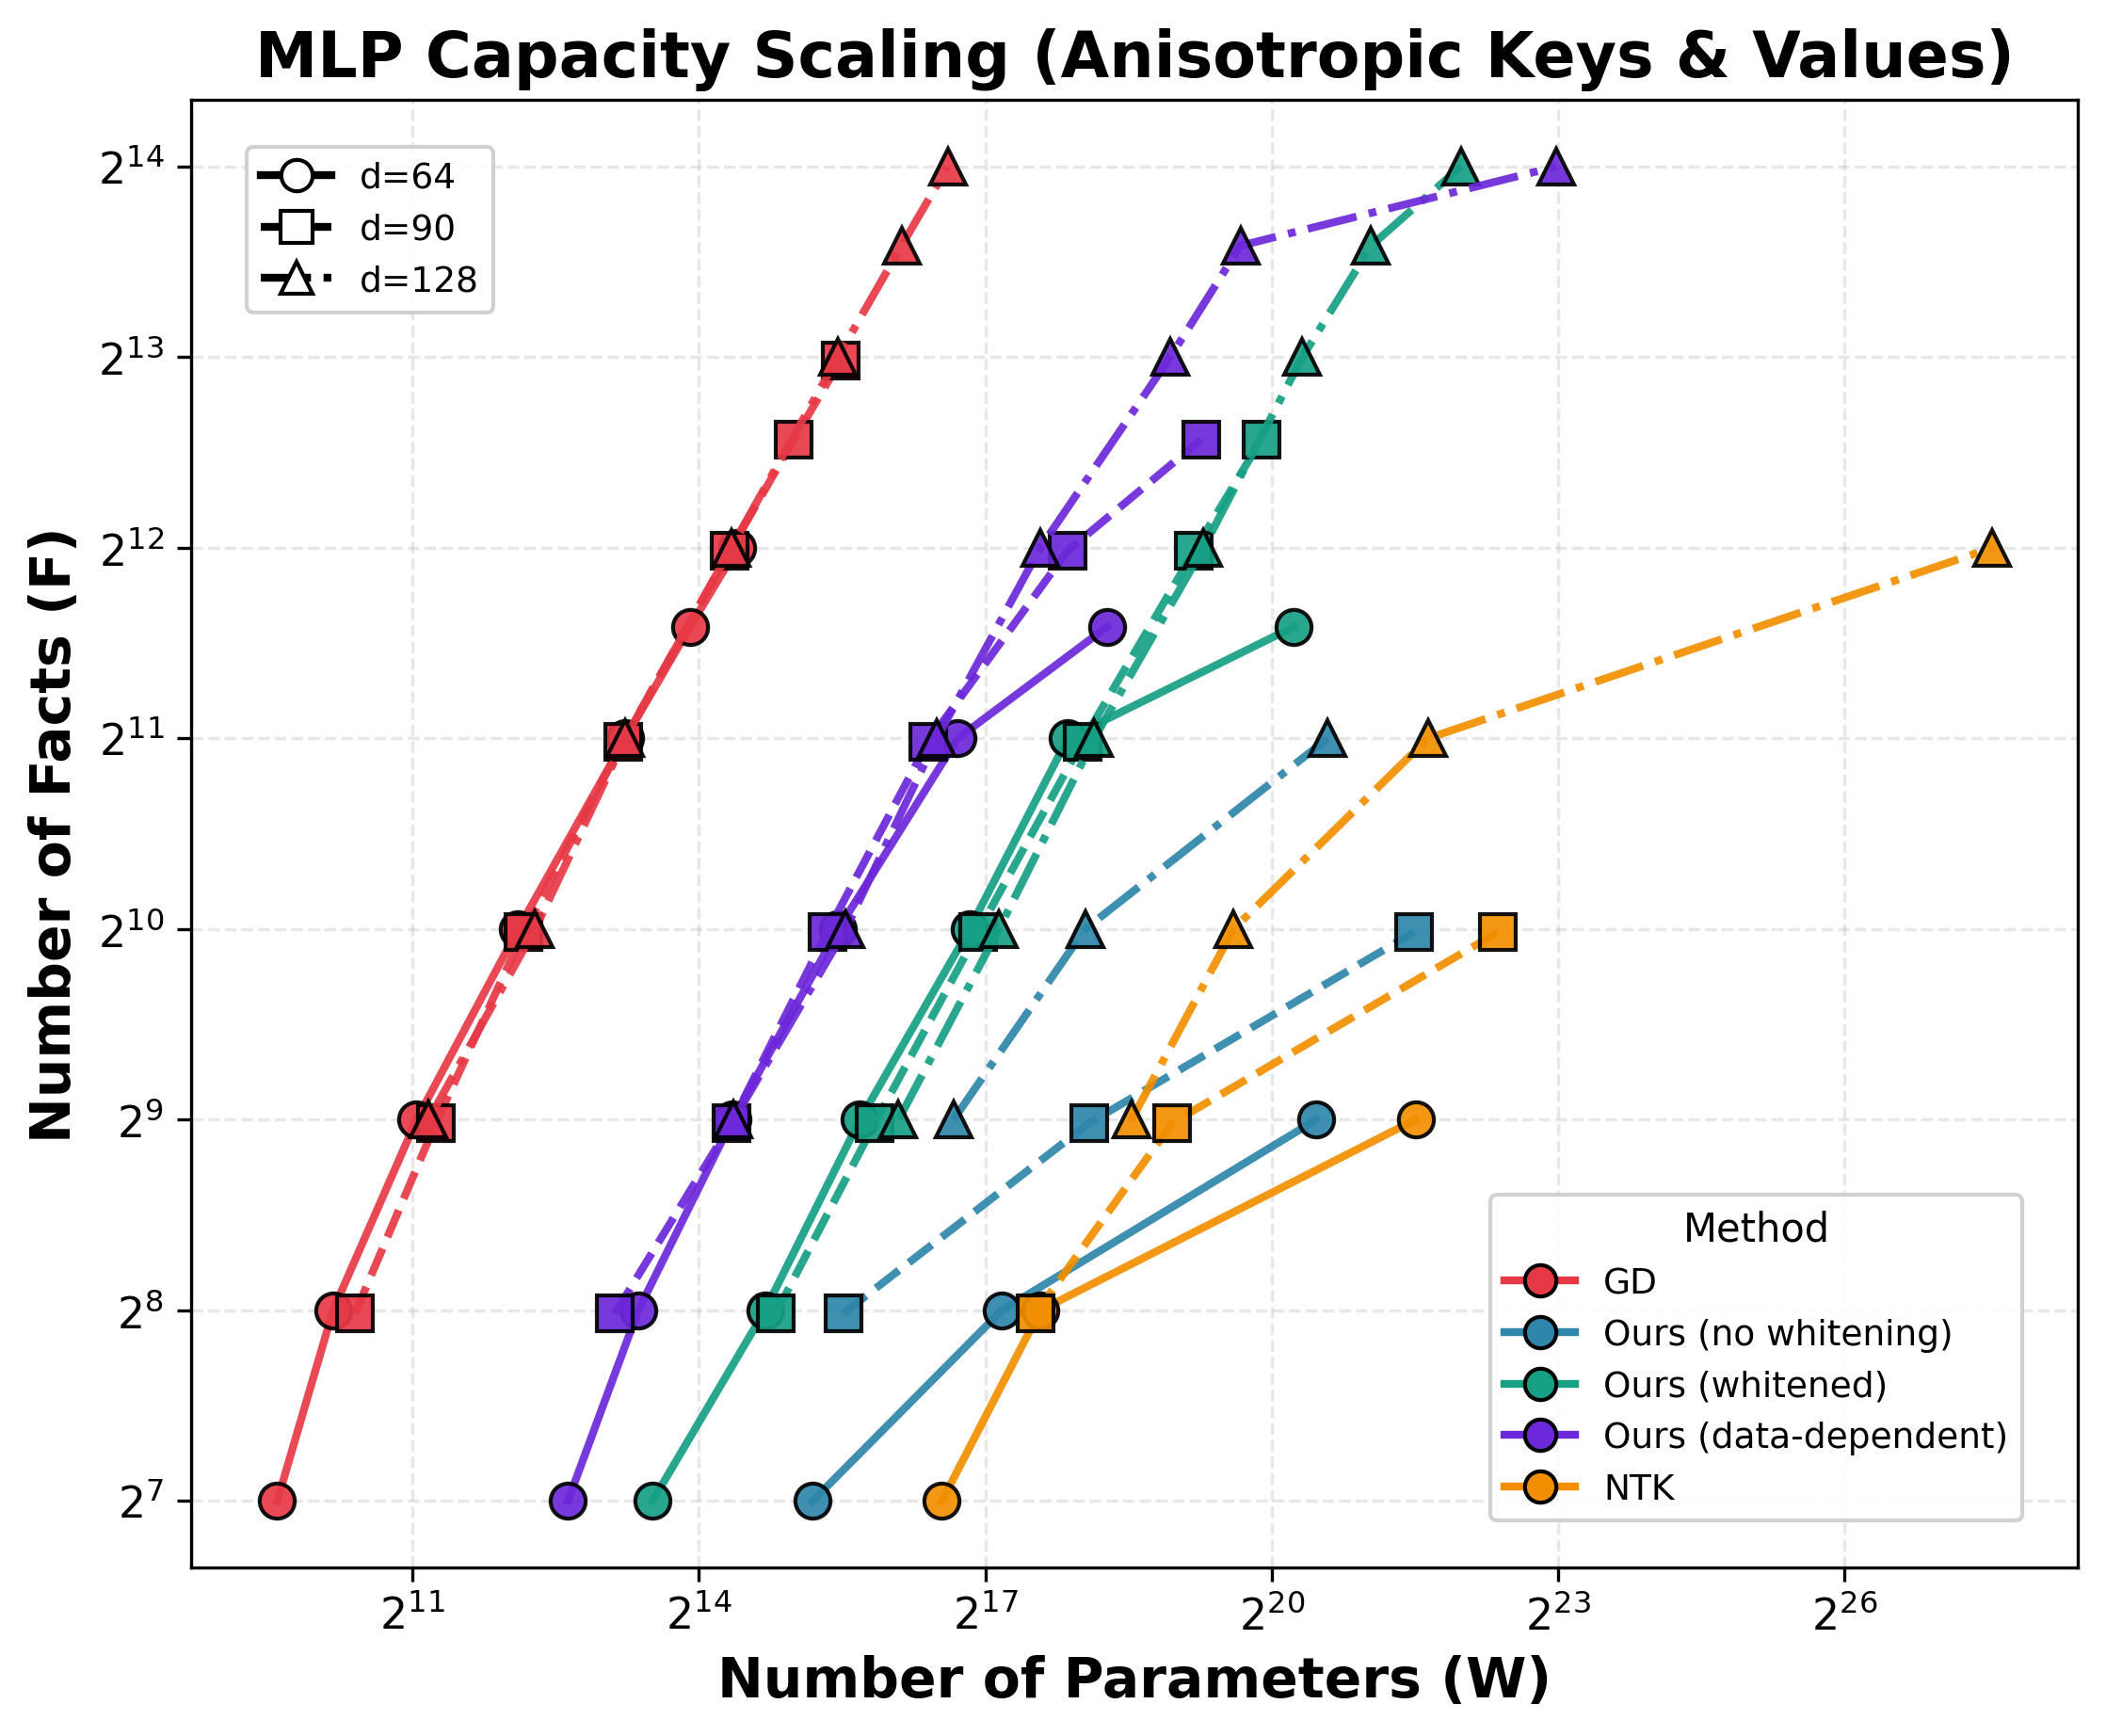
\includegraphics[width=0.86\linewidth]{sections/section_4_hebbian_kernel_mlps/figs/mlp_capacity_anisotropic_beta1p5_both_final.png}
\caption{\textbf{MLP fact-storage capacity under anisotropic keys and values.}
Our data-dependent construction achieves asymptotically optimal fact-storage capacity (only $4$-$8\times$ worse than GD), while NTK fails to achieve the desired \(W=\Theta(F\log F)\) scaling under anisotropy.}
\label{fig:appendix:anisotropic-mlp-capacity}
\end{figure}

Although anisotropic embeddings degrade the attainable fact-storage capacity for all methods relative to the isotropic setting (Figure~\ref{fig:sketched_k2_sweeps}c), our data-dependent construction remains only \(4\)–\(8\times\) worse than GD, as in the isotropic case.
On the other hand, the NTK and unwhitened constructions struggle to store facts at the \(W=\Theta(F\log F)\) scaling once both keys and values are anisotropic. We find that whitening improves fact-storage capacity substantially more in the anisotropic case.

\subsubsection{Margin and Capacity Scaling Under LLM Embeddings}
\label{app:exp:additional:llm-embeddings}

In this section, we explore the margin scaling and MLP and Transformer Block capacity scaling when using our construction on embeddings sampled from an intermediate LM layer. Concretely, we replace the synthetic spherical key/value embeddings used in Sections~\ref{sec:4}~and~\ref{sec:5} with paired \((\mathbf{x}, \mathbf{y})\) embeddings captured from a real language model. The intent is to check that the margin bounds and the predicted storage-capacity scaling remain meaningful when the keys and values come from those that an intermediate layer of an LM presents to its MLP blocks.

\paragraph{LM embeddings.} We stream the train split of WikiText through Qwen3-0.6B-Base and, at the middle decoder block (layer 14 of 28, the ``mid layer''), record per-token MLP inputs \(\mathbf{x}\) (post-RMSNorm hidden state) and outputs \(\mathbf{y}\) (pre-residual), keeping \(N=500{,}000\) pairs. A factset of size \(F\) is then built by uniformly sampling \(F\) of these \((\mathbf{x}_i, \mathbf{y}_i)\) pairs, taking \(\mathbf{x}_i\) as the input and \(\mathbf{y}_i\) as the output embedding under the identity mapping.

\paragraph{Margin scaling.} \Cref{fig:appendix:llm-margin} shows the Section~\ref{sec:4} margin scaling sweep on the captured Qwen3 mid-layer embeddings. We construct our bilinear random-feature Hebbian variant with \(d=M=1024\), sweeping \(F\) from \(4\) to \(128\) over five seeds per point. In both the arbitrary-keys/values and the isotropic regimes, the fitted bound tracks the empirical minimum margin \(\gamma_{\min}\) closely (\(R^2\geq0.95\)), suggesting that our margin scaling laws continue to hold on real, anisotropic LM embeddings.

\begin{figure}[t]
\centering
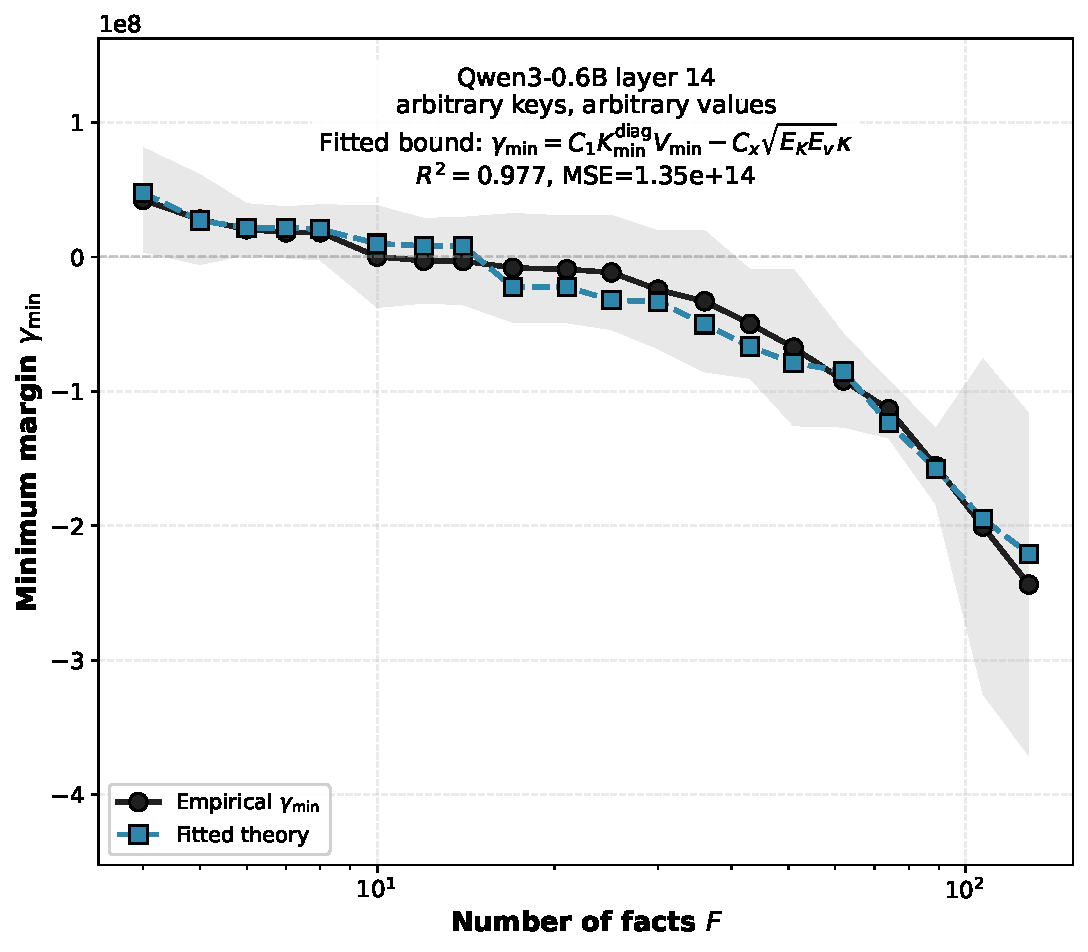
\includegraphics[width=0.48\linewidth]{sections/section_4_hebbian_kernel_mlps/figs/margin_llm_qwen3_06b_layer14_akav.pdf}\hfill
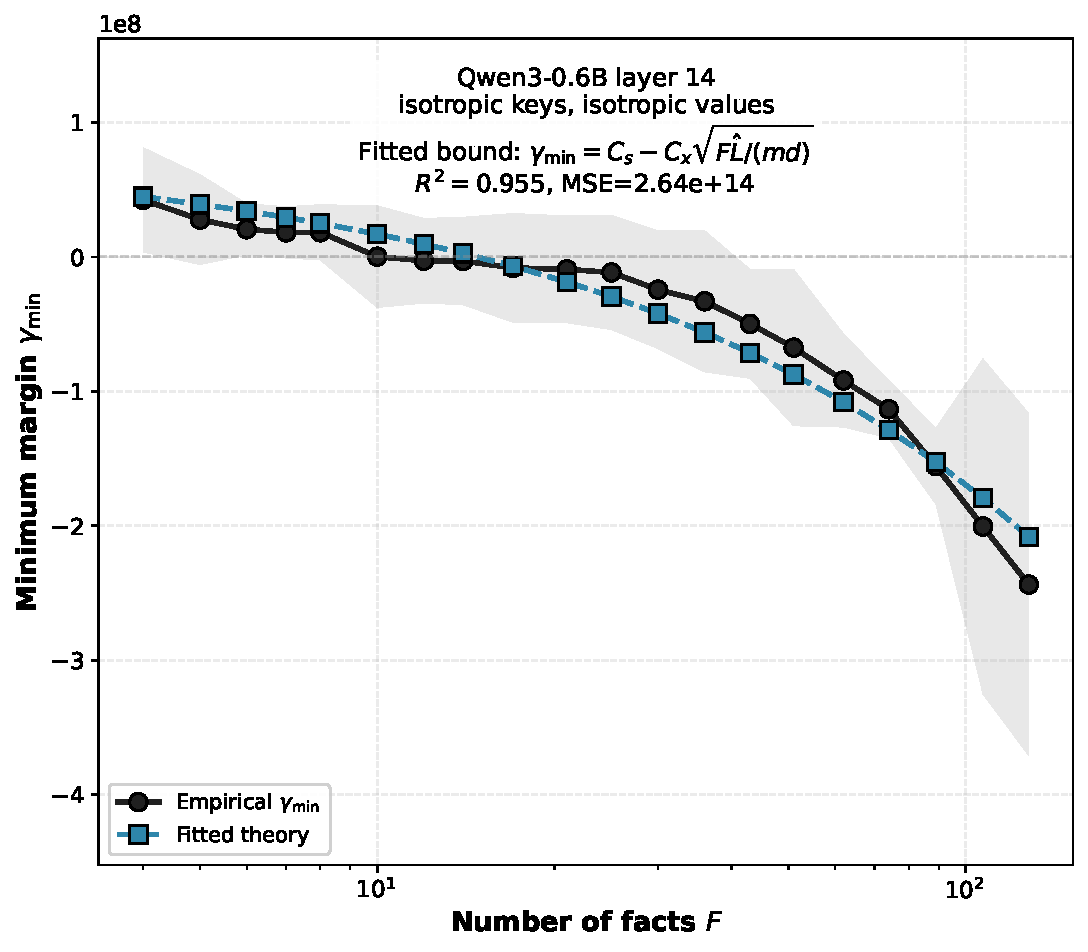
\includegraphics[width=0.48\linewidth]{sections/section_4_hebbian_kernel_mlps/figs/margin_llm_qwen3_06b_layer14_rkrv.pdf}
\caption{\textbf{Bilinear-RF margin scaling on Qwen3-0.6B mid-layer embeddings.}
Left: arbitrary keys and values, where the measured margin tracks the deterministic bound through the key/value-geometry terms $K_{\min}^{\mathrm{diag}}$, $E_K$, $E_v$ and the composite cross-talk scale $\sqrt{E_K}\sqrt{E_v}\,\kappa$. Right: the isotropic-key / isotropic-value bound, where the margin follows the single cross-talk term $\sqrt{FL/(md)}$. In both regimes the bound tracks the empirically measured minimum margin $\gamma_{\min}$ ($R^2\geq0.95$), suggesting that our margin scaling laws hold for LM embeddings.}
\label{fig:appendix:llm-margin}
\end{figure}

\paragraph{MLP storage capacity.} \Cref{fig:appendix:llm-mlp-capacity} reproduces the standalone-MLP fact-storage capacity scaling of Section~\ref{sec:4}, but with the random key/value embeddings replaced by the captured Qwen3 mid-layer embeddings. Following the protocol in Appendix~\ref{app:exp:section4:capacity}, we binary-search over MLP hidden width \(W\) for the minimum width that achieves a \(98\%\) per-fact recall threshold using our whitened bilinear-RF Hebbian construction for \(F \in \{2^9, 2^{10}, \dots, 2^{14}\}\). Notably, the facts \(F\) vs.\ parameters \(W\) scaling follows the predicted \(W \approx \Theta(F\log F)\) capacity scaling on LM embeddings.

\begin{figure}[t]
\centering
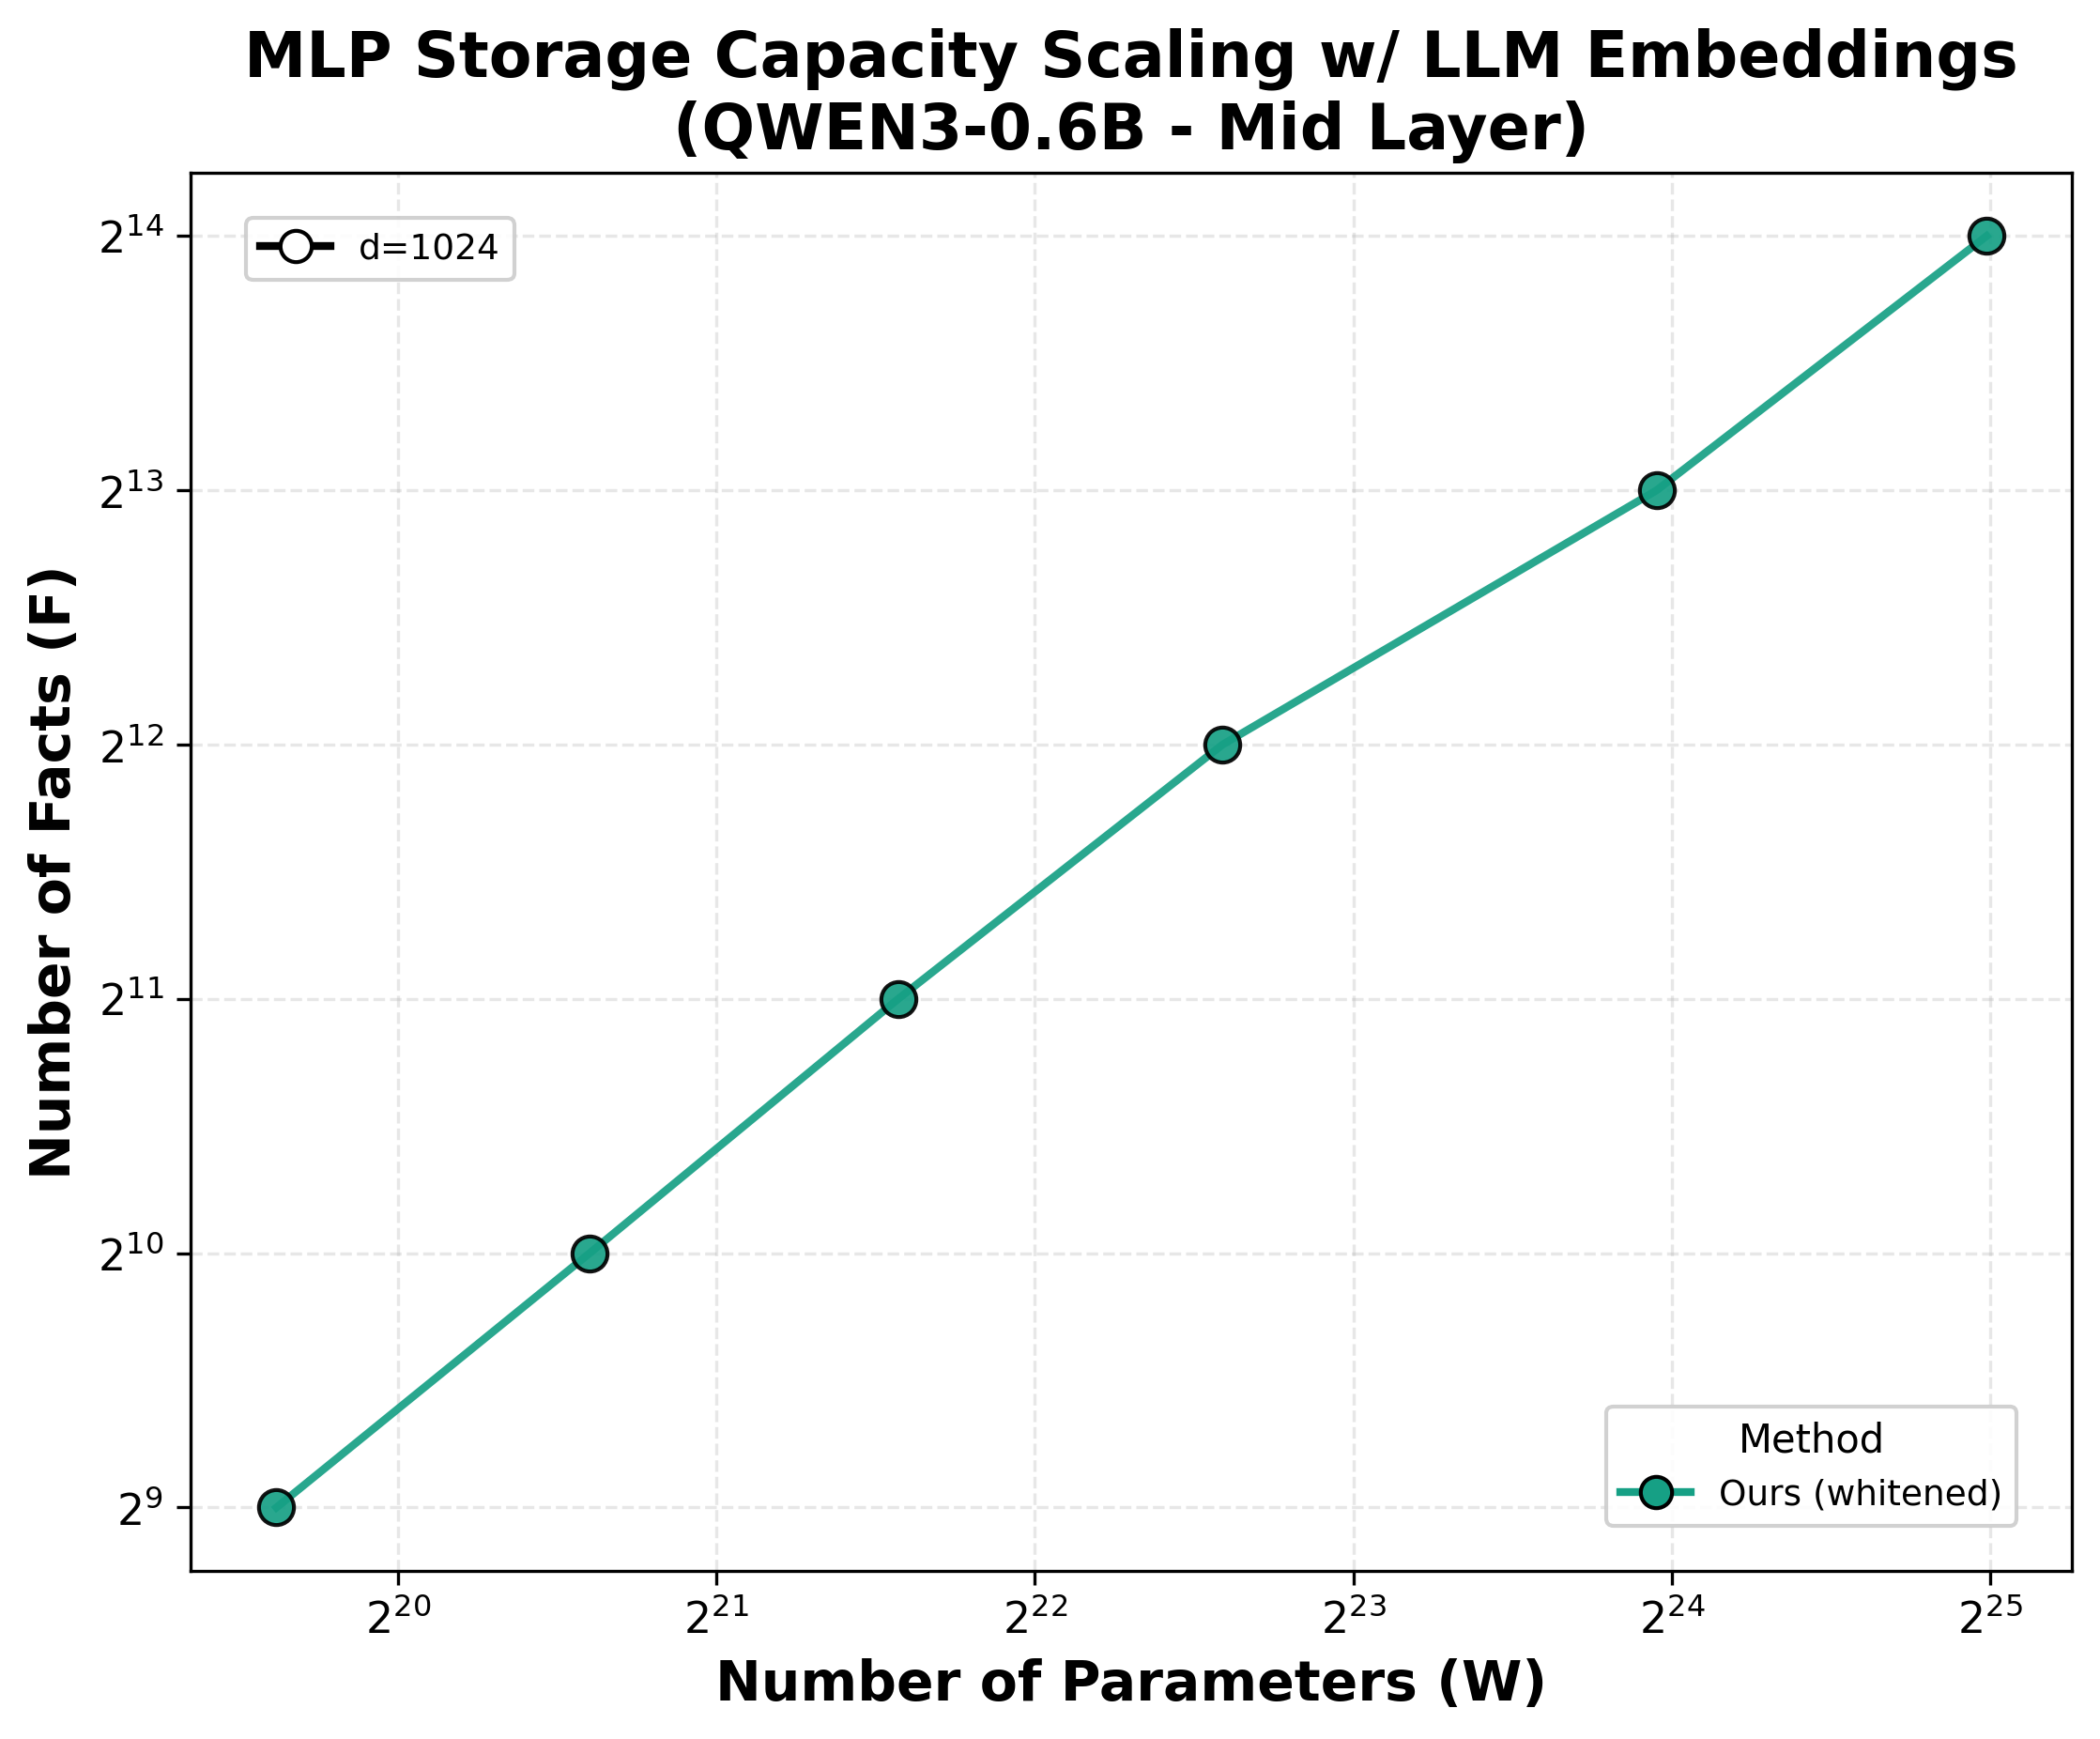
\includegraphics[width=0.62\linewidth]{sections/section_4_hebbian_kernel_mlps/figs/mlp_capacity_llm_qwen3_06b_layer14_whitened.png}
\caption{\textbf{Standalone-MLP fact-storage capacity on Qwen3-0.6B mid-layer embeddings.}
Our whitened bilinear-RF construction achieves the expected \(W \approx \Theta(F\log F)\) capacity scaling on LM embeddings.}
\label{fig:appendix:llm-mlp-capacity}
\end{figure}

\paragraph{Transformer block storage capacity.} For the Transformer block (\Cref{fig:appendix:llm-transformer-capacity}), we use the same insert-then-train-attention hidden-width capacity sweep as the main-text Figure~\ref{fig:main-figure}c: a frozen whitened-construction MLP is inserted into a single Transformer block whose input and output embeddings are the captured Qwen3 \(\mathbf{x}\) and \(\mathbf{y}\), and we binary-search for the smallest hidden width reaching the success threshold. Here, we require \(100\%\) SSFR \emph{training} accuracy on the trained fact set rather than fact-adaptive evaluation accuracy. Moreover, we keep the post-attention residual (rather than disabling it), leave the value/output projections trainable (rather than freezing them to identity), and evaluate on the same inserted MLP (rather than swapping in an eval-MLP for a held-out fact set). Notably, as in the MLP case, the facts \(F\) vs.\ parameters \(W\) scaling follows the predicted \(W \approx \Theta(F\log F)\) capacity scaling on LM embeddings.

\begin{figure}[t]
\centering
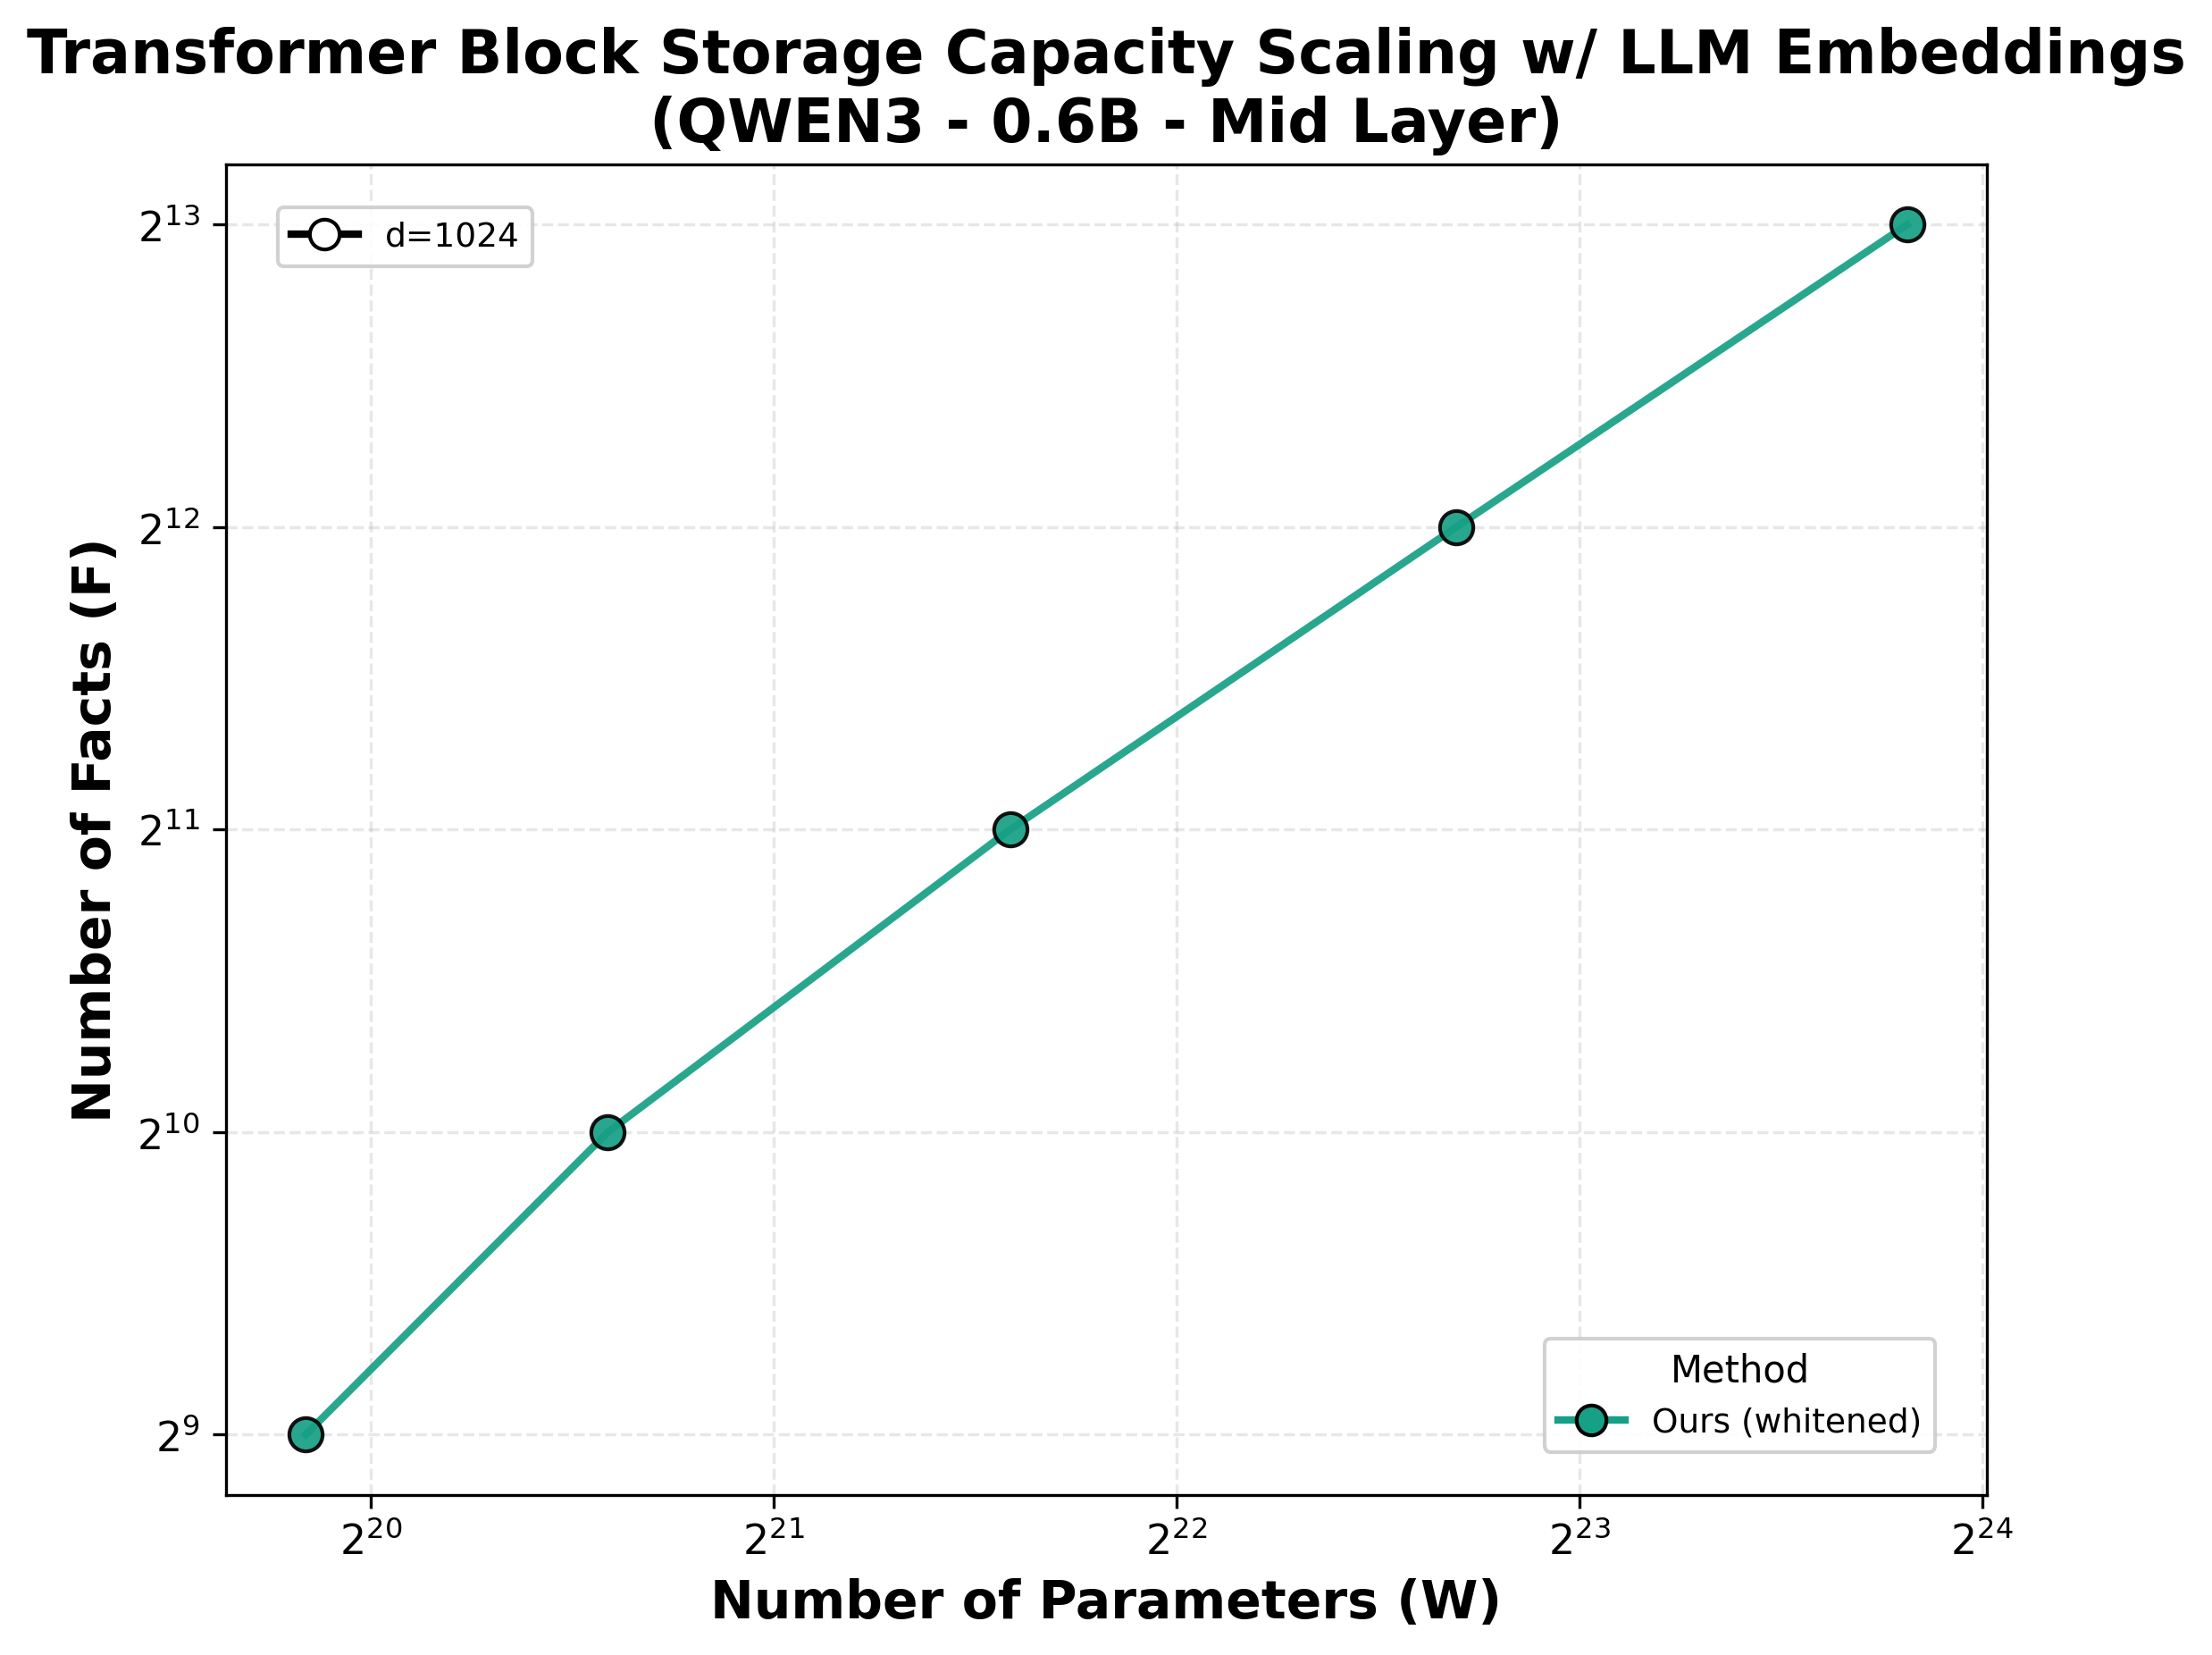
\includegraphics[width=0.62\linewidth]{sections/section_5_transformer_integration/figs/transformer_capacity_llm_qwen3_06b_layer14.png}
\caption{\textbf{Transformer-block fact-storage capacity on Qwen3-0.6B mid-layer embeddings (training-accuracy criterion).}
Our whitened bilinear-RF construction, inserted into a full Transformer block, retains the expected \(W \approx \Theta(F\log F)\) scaling on LM embeddings.}
\label{fig:appendix:llm-transformer-capacity}
\end{figure}
